\documentclass{article}
\usepackage{graphicx}
\begin{document}
	\section*{Table}
	\begin{tabular}{|l|r|r|r|} \hline
		Course & Student1 & Student2 & Student3   \\\hline
		CS100 & 77 & 56 & 99 \\ \hline
		CS101 & 45 & 34 & 77 \\ \hline
		CS102 & 97 & 68 & 24 \\ \hline
		CS103 & 22 & 89 & 38 \\ \hline
		CS104 & 72 & 96 & 88 \\ \hline
	\end{tabular}
	
	\section*{Linepoints}
		\begin{figure}[h]
			\centering
			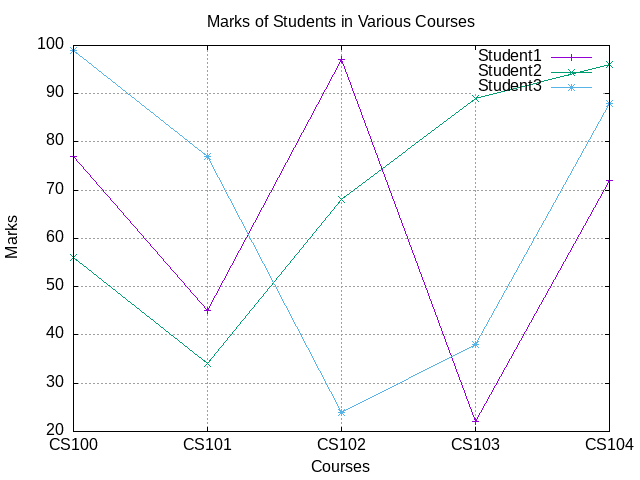
\includegraphics[width=0.7\linewidth]{Linespoint}
			\caption{}
			\label{fig:linespoint}
		\end{figure}

	\section*{Histogram}
		\begin{figure}[h]
			\centering
			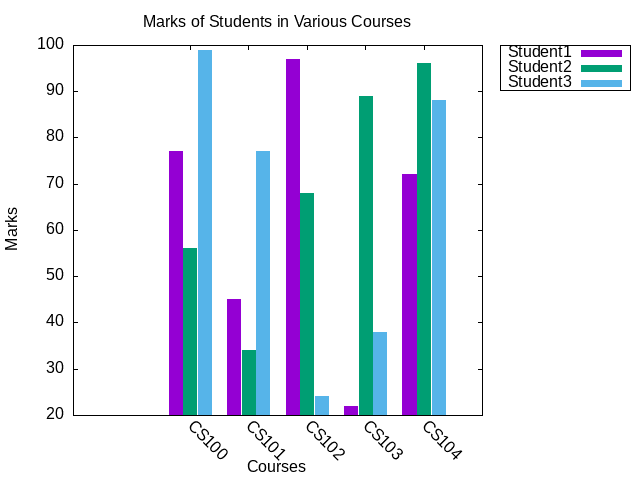
\includegraphics[width=0.7\linewidth]{Histogram}
			\caption{}
			\label{fig:histogram}
		\end{figure}

	\section*{StackHistogram}
		\begin{figure}[h]
			\centering
			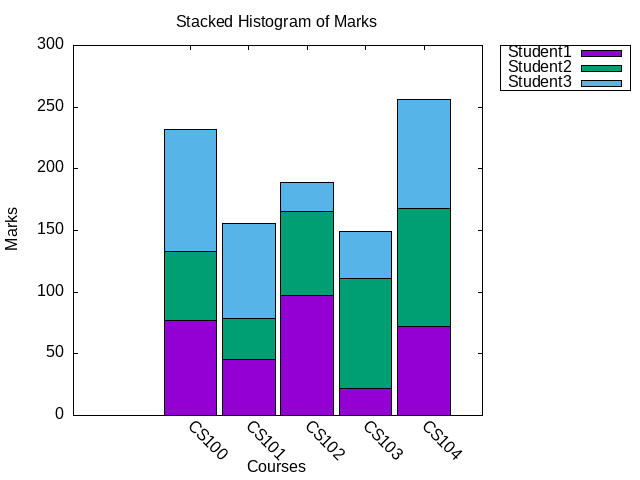
\includegraphics[width=0.7\linewidth]{Stacked_Histogram}
			\caption{}
			\label{fig:stackedhistogram}
		\end{figure}

		
\end{document}